\documentclass[12pt]{article}
\usepackage[francais]{babel}
\usepackage[utf8]{inputenc}
\usepackage{graphicx}
\usepackage{amsmath}
\usepackage{amsfonts}
\usepackage{amssymb}




\addtolength{\hoffset}{-1cm}
\addtolength{\textwidth}{2cm} 
\addtolength{\voffset}{-1cm}
\addtolength{\textheight}{2cm} 

\begin{document}

\begin{titlepage}
\begin{center}

\hfill
\vfill
\bigskip
\huge{ 
\includegraphics[width=60,height=50]{logo.png} 

\includegraphics[width=80,height=50]{lh.png} \\
 Rapport de stage \\ M2 MATIS  \\ \\ \\ \\ \\
 } 
\vfill
\bigskip 
\Huge 
\bigskip 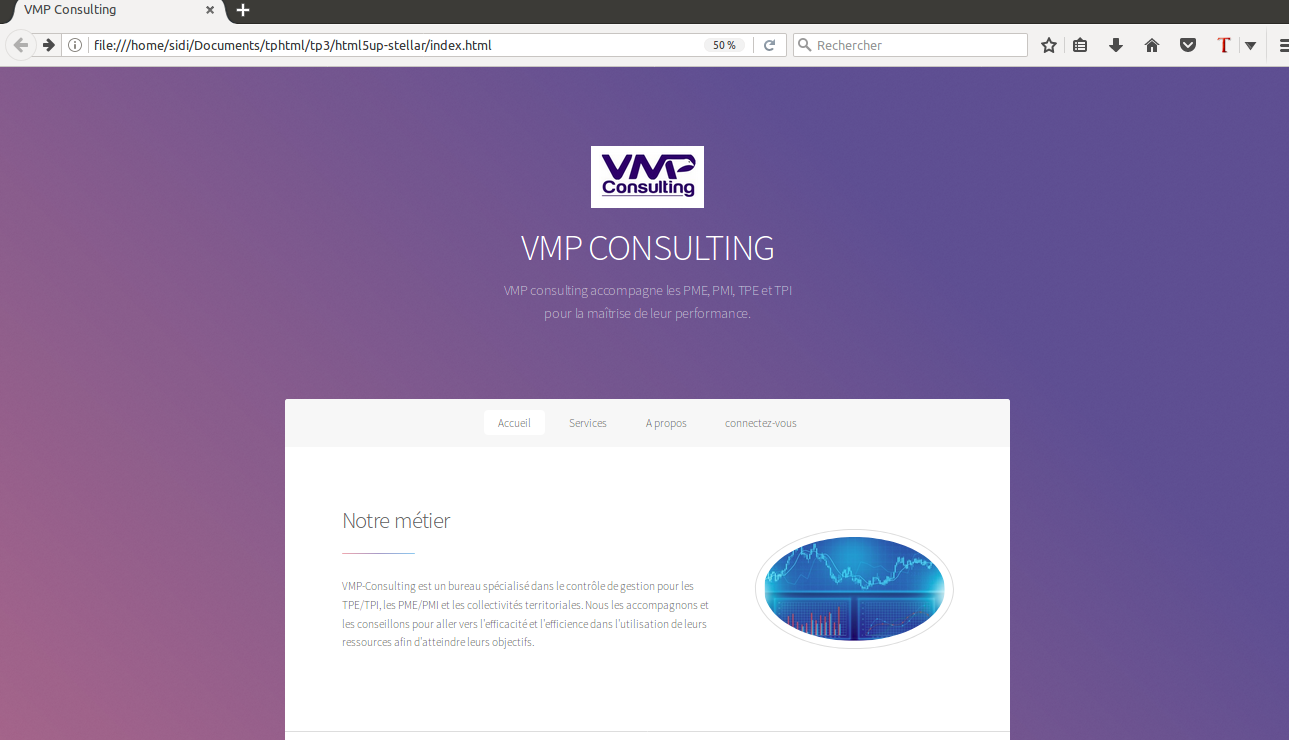
\includegraphics[width=120,height=150]{design1.png}} \\ \\
 Développement d'un portail web collaboratif sous Symfony 3 \par 
\vfill

\Large \begin{flushleft}
 Réalisé par:\\ sidi Maouloud \par
\end{flushleft}
		 
		  \begin{flushright}
		                    sous la direction de:\\  M. ould Maouloud
		                   \end{flushright}



		 
\vfill
\Large Université du Havre \par \Large VMP Consulting		
		\bigskip 
\bigskip

\Large
Juillet-Novembre 2017
\end{center}
\end{titlepage}

\section*{Remerciements}
Je tiens á transmettre ma gratitude et mon affection à ma mère, mon père  et ma
sœur, ainsi que mes proches pour leur patience et leur soutien.\\ \\

J’adresse mes remerciements à  M. sidi ould MAOULOUD, de m’avoir accueillie pour faire mon
stage au sein de son entreprise, ainsi pour son aide et  ses  remarques pertinentes.  \\ \\
J’aimerais aussi remercier M. Laurent Amanton  et tous mes enseignants de l’université du havre
qui m’ont accompagné 
au cours de cette année.\\ \\


\newpage

\section*{Résumé}
\textbf{VMP-CONSULTING}  est un bureau spécialisé dans le contrôle de gestion pour les TPE/TPI, les PME/PMI et les collectivités territoriales. Il les accompagne et les conseille pour aller vers l'efficacité et l'efficience dans l'utilisation de leurs ressources afin d'atteindre leurs objectifs.\\
Pour mieux servir ses clients, \textbf{VMP-CONSULTING}  veut avoir un portail web pour 
mettre en œuvre un espace de travail unique pour les clients, 
 proposer aux clients un accès privilégié et personnalisé à divers services en
ligne, et 
développer des outils qui permettent aux clients de réagir avec les contenus du
portail.\\
L'objectif de ce stage est de réaliser ce site web.


\section*{Abstract}
Whatever the activity, today all companies are confronted with increased competitive pressure, technological changes ... To enable managers and operational staff to devote themselves entirely to their core business, support in managing The company is a necessity not to say an obligation. In this area, not all businesses are housed in the same category, particularly small businesses and small businesses. The lack of management tools is mainly linked to a problem of means although sometimes it can be a problem of awareness of the utility and the benefit brought by these tools.\\
\textbf{VMP-CONSULTING}  is an office specializing in management control for small and medium-sized enterprises (SMEs), SMEs and local authorities. He accompanies them and advises them to move towards efficiency and efficiency in the use of their resources in order to achieve their objectives.\\
To better serve its customers, \textbf{VMP-CONSULTING}  wants to have a web portal for
implement a unique workspace for customers,
 offer customers privileged and personalized access to various services in
line, and
develop tools that enable clients to react with the contents of the
portal.\\
The objective of this traineeship is to realize this website

\newpage

\tableofcontents
\newpage



\section{Introduction}

Un portail web est une plate-forme collaborative dont la fonction première est de proposer aux internautes des ressources et services numériques en rapport avec un thème, un domaine d’intérêt et dédié à chaque communauté particulière (les collaborateurs, les partenaires, les clients ou encore les fournisseurs …).\\
Il s’agit d’un espace de travail unique, personnalisé et sécurisé avec des droits d’accès par utilisateur.\\
L’enjeu pour une entreprise aujourd'hui est d’adresser une communication ciblée en proposant un contenu pertinent à l’utilisateur, par exemple, mettre en avant tous ses produits et offres complémentaires permet d’informer ses clients et de déclencher de nouvelles ventes.\\ \\



En effet, les clients n’ont pas forcément le réflexe de consulter le site internet ou les newsletters de leurs prestataires pour s’informer de leurs actualités. Le portail web devient ainsi un relais d’information et de suivi commercial auprès des clients.\\ Un portail web  permet de  Capitaliser les informations et les savoir-faire,
    simplifier la recherche d’informations,
    centraliser l’ensemble des données en un seul accès et
    fédérer les collaborateurs et les utilisateurs autour de l’entreprise.
\\
Généralement, les sociétés ont des portails web respectant leur charte graphique pour être en cohérence avec leur image de marque. Le client habitué de la marque étant dans le même univers, il assimilera plus facilement la plateforme collaborative de l’entreprise.\\

 \\
 
 \subsection{Problématique}
Pour un bureau d’études, comme \textbf{VMP-CONSULTING} , il s’agit de mettre en avant tous leurs panels de prestations : de l’étude à la formation en passant par la maîtrise d’œuvre.\\
Pour cela \textbf{VMP-CONSULTING} , qui est spécialisé dans le contrôle de gestion pour les TPE/TPI, les PME/PMI et les collectivités territoriales, veut mettre en place un site web(Portail web) dédié à ses clients pour :\\

\begin{itemize}

\item  Dynamiser la collaboration avec les interlocuteurs internes et externes
 \item   Permettre la transmission des connaissances pour une organisation plus productive et performante
 \item     Améliorer le suivi des prestations réalisées par les consultants techniques : suivre en temps réel les interventions chez les clients afin d’accélérer la prise en charge directement depuis le terrain, disposer d’indicateurs et de statistiques pour détecter les problèmes récurrents.
 
 \item   Renforcer  l'offre auprès des clients, les fidéliser avec de nouveaux services
 \item   Optimiser certaines tâches back-office : accès aux données et à l’historique des  clients, avancement des taches, ...
\item    Répondre à de nouvelles exigences et garder une longueur d’avance.

\end{itemize}

\\

L’objectif de ce stage est de répondre à ces problématiques en réalisant un portail web qui permettra
 à \textbf{VMP-CONSULTING} de bien satisfaire ses clients(Traçabilité des échanges de fichiers, Planning, Tableaux de bord graphiques, plans, schémas, études, et indicateurs de pilotage...).\\
Ainsi un portail web bien conçu permet d’améliorer la productivité des collaborateurs et la fidélité des clients.
Ceci oblige donc une bonne conception du projet et  l'utilisation par la suite  des  outils et technologies efficaces permettant  
 le succès du site web.\\ 


\subsection{VMP Consulting}


Quelle que soit l’activité, aujourd’hui toutes les entreprises sont confrontées à une pression concurrentielle accrue, aux évolutions technologiques...Pour permettre aux managers et aux opérationnels de se consacrer entièrement à leur coeur de métier, un accompagnement dans la gestion de l'entreprise est une nécessité pour ne pas dire une obligation. Dans ce domaine là, les entreprises ne sont pas toutes logées à la même enseigne, en particulier les TPE et certaines PME. Le manque d’outils de gestion est principalement lié à un problème de moyens même si parfois il peut s’agir d’un problème de sensibilisation à l’utilité et le bénéfice apporté par ces outils.\\ \\

VMP-Consulting est un bureau spécialisé dans le contrôle de gestion pour les TPE/TPI(trés petite entreprise), les PME/PMI(petite moyenne entreprise) et les collectivités territoriales. Il les accompagne et les conseille pour aller vers l'efficacité et l'efficience dans l'utilisation de leurs ressources afin d'atteindre leurs objectifs.\\ \\


VMP Consulting accompagne les PME, PMI, TPE et TPI pour la maîtrise de leur performance, avec ses solutions, pour atteindre les objectifs de :
\begin{itemize}

\item Maîtriser les coûts.

\item Optimiser les performances.

\item Une transparence sur la gestion des ressources de  l'entreprise.

\item Le développement de la réactivité dans la prise de décisions stratégiques.
\end{itemize}
\\ \\ 


Parmi ses services :
\begin{itemize}

\item \textbf{Pilotage d'entreprise: } Des conseils en gestion et pilotage d'entreprise permettent aux managers et aux opérationnels de disposer d’un système de contrôle de la performance et d’aide à la décision.


\item \textbf{Audi: } Un audit qui permet de donner une situation précise de l'entreprise, un
diagnostic qui  permettra de développer les activités, gérer efficacement les risques et prendre les bonnes décisions stratégiques dans les meilleures conditions.


\item \textbf{Système d'information : }  Assistance à la maîtrise d’ouvrage et accompagnement du changement,
 Coordination et gestion de projets, 
 Elaboration des cahiers de charges et des spécifications fonctionnelles, 

 Audit de systèmes d’informations, et

Elaboration d’outils spécifiques.


\item \textbf{Formations: } VMP apporte toute son expérience pour des formations qui permettrons de maîtriser tous les outils nécessaires à la bonne marche de l'entreprise.
\end{itemize}
\\ \\ 



Le créateur du startup a une expérience de plus de 20 ans dans divers secteurs d'activités et dans plusieurs types de structures (PME - Multinationales - Organismes d'Etat), et en 2016 il a lancé VMP CONSULTING.




\subsection{Cahier de charges et Objectifs}

Comme tout projet professionnel, le début de ce stage était d'abord à définir la 
problématique,  pour passer par la suite à la rédaction du cahier des charges, en 
traçant  les grandes lignes du projet, et les objectifs à atteindre.\\ 

Le besoin d'un portail web pour \textbf{VMP-CONSULTING}, vient des enjeux suivants: \\

\begin{itemize}
\item Améliorer la productivité des services de l'entreprise.
\item Fidéliser les clients.
\item Se différencier par rapport à la concurrence en proposant un panel de services à
valeur ajoutée.
\item Conquérir de nouveaux clients.
\end{itemize}

\\

Ainsi les objectifs principales de ce stage sont incarnés par  :\\
\begin{itemize}
\item Mettre en œuvre d'un espace de travail unique pour les clients.
\item Proposer aux clients un accès privilégié et personnalisé à divers services en
ligne.
\item Développer des outils qui permettent aux clients de réagir avec les contenus du
portail.
\item Suivre en temps réel l'ensemble des tableaux des bords et d'indicateurs des performance.
\item Faire des prévisionnels, saisir des hypothèses d'évolutions des indicateurs de gestion  et calculer des projections 
de résultat.

\end{itemize}

 Ceci passe par: \\
\begin{itemize}
\item La réalisation d'une maquette et des templates   .
\item La réalisation des développements, test et recettes fonctionnelles.
\item  La mise en place de l'hébergement.
\end{itemize} \\

Après la mise en point sur les besoins, on peut passer à la rédaction du cahier des charges fonctionnel .\\
Par exemple :\\
\begin{center}
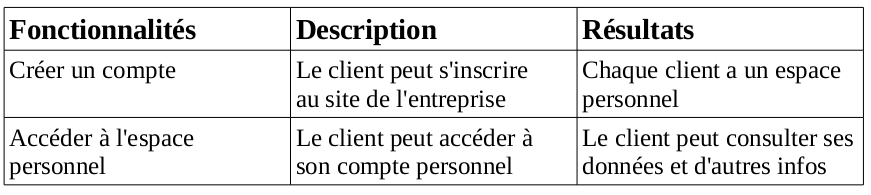
\includegraphics[width=200,height=250]{cdc2.png}}
\end{center}
 \\ \\
 

\subsection{Environnement et Missions}

 \textbf{VMP-CONSULTING} veut réaliser ce projet à l'aide d'un développeur web qui va être sous 
sa direction, le projet est piloté et suivi  par le dirigeant du bureau d'études.
Ce stage a déroulé 4 mois, de juillet à Novembre au sein de la société à Boves(Amiens, région Picardie ).

Mes missions en tant que le seul développeur du projet sont : \\
\begin{itemize}
\item Analyse des données et proposition des solutions .
\item Conception et modélisation  du site web et de la bases de donnée.  
\item Développement du portail web.
\item test et déploiement du site internet.
\end{itemize}

\begin{center}
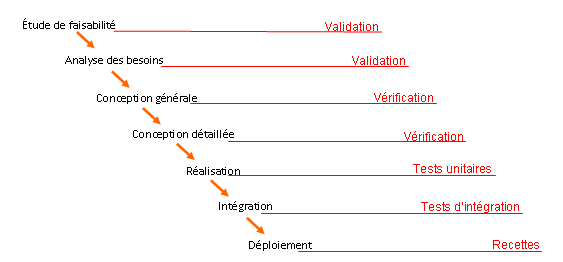
\includegraphics[width=300,height=250]{p.png}}

\end{center}


On verra tout au long du rapport toutes ces détails. 


\newpage

\section{Analyse et Conception}
L'objectif final de ce projet est de réaliser une plat-forme web collaborative facilitant le contrôle des gestions 
pour les entreprises clientes.\\
Pour cela  une analyse, des méthodes et des données des entreprises, est  nécessaire pour concevoir et implémenter
 le système d'information de gestion qui est une partie principale du portail web.


\subsection{Contrôle et système d'information  de gestion}
Le Contrôle de gestion est le garant de la bonne santé de la structure en s'assurant que les ressources sont employées efficacement.\\

Il intervient également pour fournir les outils qui vont servir aux décideurs pour suivre l'impact de leurs actions. Celles-ci résultant de décisions de portées stratégiques et tactiques.\\

Dans de nombreuses entreprises, il est en charge du management du système de pilotage avec la prise en charge des tableaux de bord destinés à la direction et aux responsables opérationnels.\\

\begin{center}
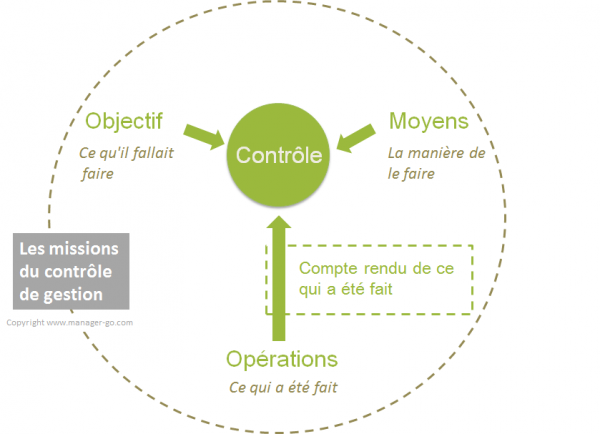
\includegraphics[width=200,height=250]{g.png}}

\end{center}

Globalement cette fonction agit à 2 niveaux : efficacité et efficience
\begin{itemize}
\item Efficacité, en influençant l'entreprise à exploiter ses activités en cohérence avec les objectifs fixés

\item Efficience, en utilisant les moyens disponibles de la manière la plus productive 
\end{itemize}
\\
Autrement dit, ces tâches s’illustrent par :
\begin{itemize}

\item Etablir des plans à long terme et les budgets,
\item Contribuer au choix des méthodes de prévisions,
\item Etablir une coordination du processus budgétaire,
\item Faire respecter les délais,
\item Analyser les résultats,
\item Et proposer des actions correctives.

\end{itemize}

Aujourd’hui,  l’information  est  incontestablement  une  ressource  vitale  de 
l’entreprise. De plus en plus, la compétitivité de l’entreprise et sa capacité de 
mise  en  œuvre  des  stratégies  sont  en  effet  étroitement  liées  à son  système 
d’information.\\
Le  contenu  en  information  des  processus  de  production  est  essentiel  à
l’amélioration de qualité.
La rapidité de réaction est, plus que jamais, un facteur essentiel de l’aptitude 
d’une  entreprise  à faire  face  à la  concurrence ;  or  cette  aptitude  est,  pour 
une bonne part, fonction de la fluidité, de la fiabilité et de la flexibilité des 
systèmes d’information de gestion. \\ \\
Le but est donc d’intégrer dans le site web un Système  d’information  pour  les  opérationnels  destiné à leur  permettre  de 
suivre   de   manière   permanente   leurs   performances   et 
d’infléchir 
éventuellement leur action grâce à l’analyse des actions réalisées.


\subsection{Étude de l’existence}

Actuellement \textbf{VMP-CONSULTING} utilise  des outils performants et facile à manipuler 
pour faire le contrôle de gestion de ses clients.\\
Le logiciel Excel de Microsoft est parmi ces outils.Les analyses et les calculs du futur système de gestion sont basés
sur des fichiers existants en Excel.\\
\begin{center}
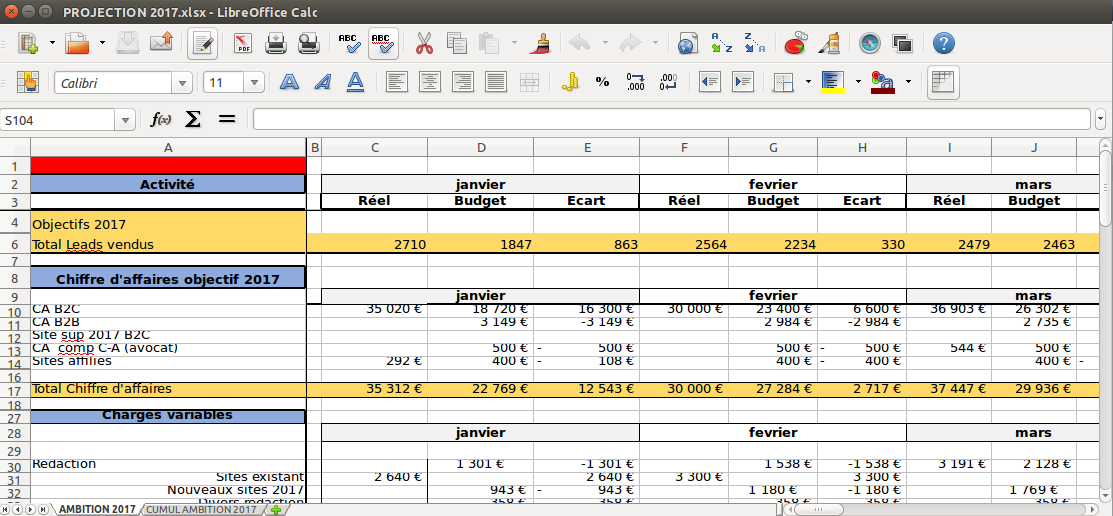
\includegraphics[width=300,height=250]{e1.png}}
\end{center}

Les données et les résultats qui contiennent ces fichiers ont été étudié attentivement afin de les transformer en 
une base de données interactive qui peut être consultée en ligne en toue sécurité, et ses données peuvent être 
visualisées en temps réel.

\begin{center}
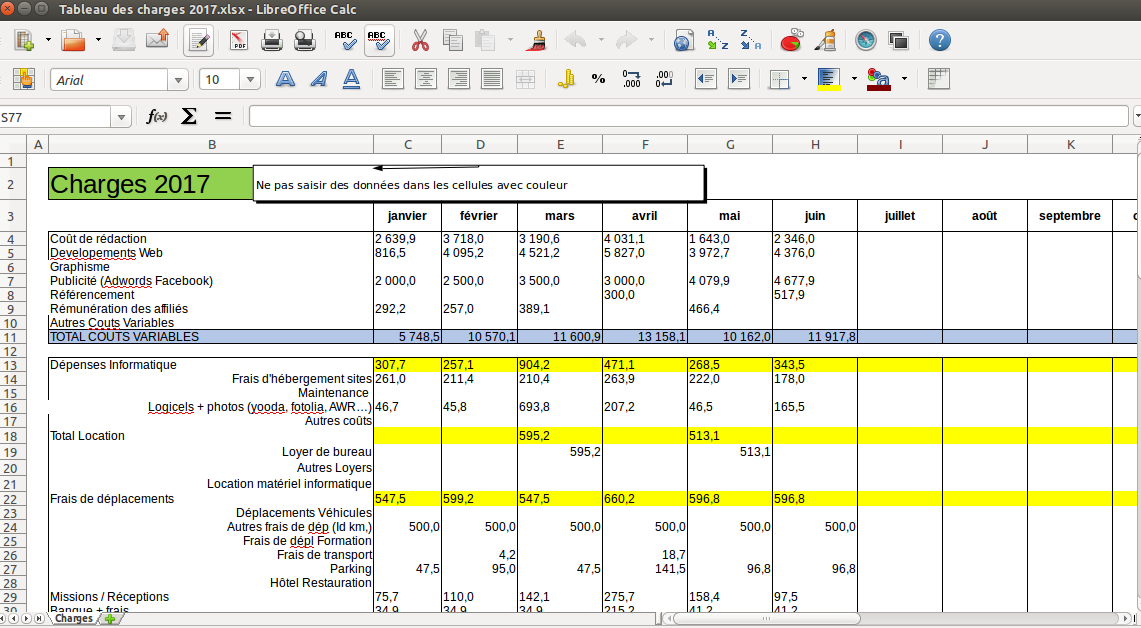
\includegraphics[width=300,height=250]{e2.png}}

\end{center}
\\

Par exemple les données du fichier excel ci-dessous représentent l'évolution du chiffre d'affaire d'une entreprise
cliente. On peut obtenir ces information dans le portail web sous forme de tableau de bord ou de simple tableau 
affiché par la jointure des différentes tables de la base de données.
\\
 
\begin{center}
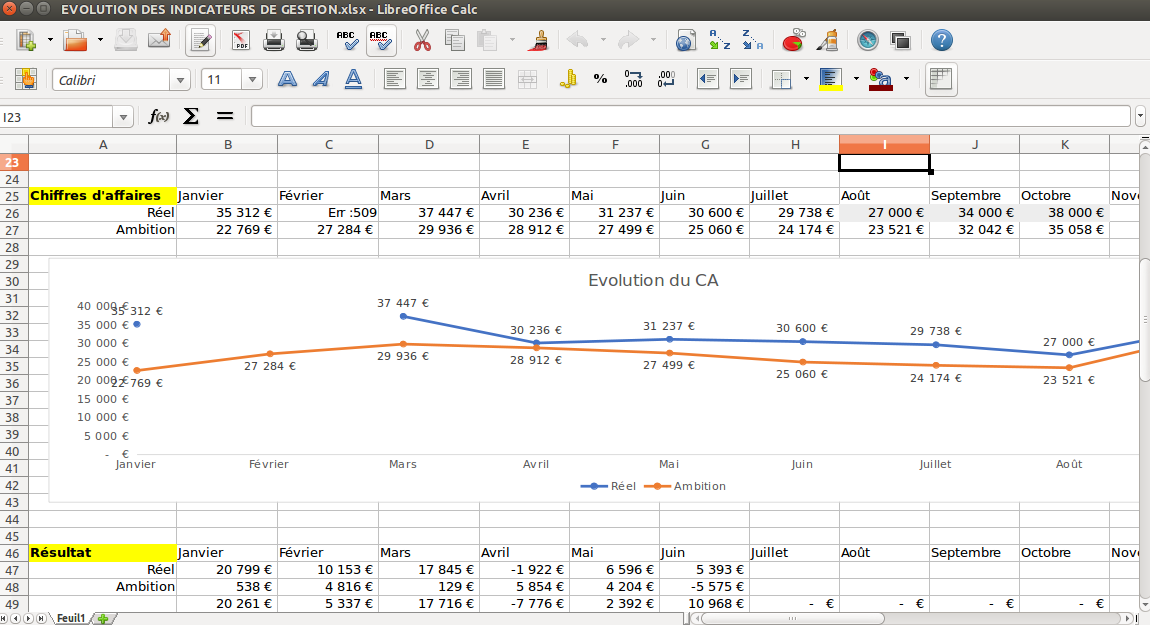
\includegraphics[width=300,height=250]{e3.png}}

\end{center}

\subsection{Outils,Technologies et Méthodes}
Après l'analyse des donnés on arrive à la pratique, mais avant cette étape
on doit préciser  les solutions à appliquer pour la résolution
des problèmes.
A noter que j'avais toute la liberté de choisir, rien n'était exigé par l'entreprise, mais à condition que 
le choix doit être bien justifié.


\subsubsection{Système d'exploitation}
Le système d'exploitation choisi est Linux avec sa distribution \textbf{Ubuntu 14.04} , il est open source, sécurisé et son
environnement est bien adapté au développement du projet. 

\subsubsection{Architectures}
Un des plus célèbres design patterns s'appelle MVC, qui signifie Modèle - Vue - Contrôleur. C'est celui que je me suis
basé pour la construction de l’architecture du site web.

Le pattern MVC permet de bien organiser son code source. Il permet de savoir quels fichiers créer, mais surtout à définir leur rôle. Le but de MVC est justement de séparer la logique du code en trois parties(Modèle - Vue - Contrôleur).\\

\begin{center}
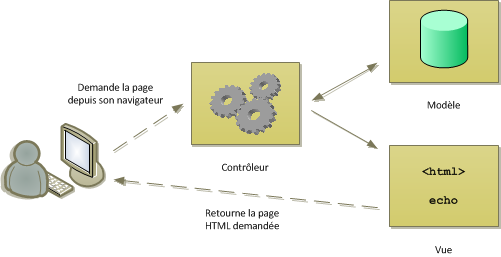
\includegraphics[width=300,height=250]{mvc.png}}

\end{center}


\subsubsection{Méthode de Programmation }

Les principales solutions existantes pour réaliser ce type de site Web sont :
\begin{itemize}
\item le codage « from scratch », c'est à dire en partant de zéro en utilisant un langage de programmation de A à Z.
\item l'utilisation d'un CMS qui  nous évite les lignes de codes .
\item l'utilisation d'un framework basée sur un langage de programmation.
\end{itemize} \\
La solution from scratch a été abandonnée, car elle est trop lourde et longue à
développer, surtout quand il s'agit d'un stage de 4 mois avec beaucoup des choses à réaliser.\\ 
Ainsi la solution CMS n'a pas été retenue puisqu'elle n'est pas adapté pour le genre de base de données interactive que 
nous souhaitons mettre en œuvre, avec la lenteur d'accès aux bases de données qui est visible surtout à l'affichage des pages
est un grand inconvénient d'un CMS.\\ \\

En revanche, l'utilisation d'un framework implique le développement sur-mesure de
tous les éléments du site à l'aide de fonctions relativement simples. L'apprentissage au
développement avec un framework apparaît plus simple qu'avec un CMS.\\

C'est pourquoi, le choix est d'utiliser un framework pour le développement du site web.\\

Mais le problème des choix ne s’arrête pas ici, il reste de préciser le choix du langage web et son framework.
 
\subsubsection{Langage web coté serveur }
Le langage de programmation utilisé va beaucoup influer sur le projet et la manière dont celui-
ci sera développé, en fonction des avantages et des inconvénients du langage.\\
On parle ici du langage back-end du site web, puisque le développement back-end est nécessaire pour bien gérer 
la bases de donnés, les  utilisateurs et les résultats à envoyer, en basant sur l'architecture MVC.\\ \\
Le choix du langage web est une autre étude qui a pris pas mal de temps en cherchant les différents langages, leurs 
avantage et inconvénients. Les recherches étaient concentrés sur les langages suivants :
\begin{itemize}
\item PHP
\item Nodejs (JavaScript back-end)
\item JavaEE

\end{itemize}

Les autres langages ont été abandonné immédiatement par le motif de manque d'une base de connaissance permettant
l'apprentissage rapide du langage.\\ \\

Le choix du langage s’est finalement porté sur \textbf{PHP} avec sa version 5(exactement 5.4.9), qui 
 est un langage
de script exécuté côté serveur. Langage élaboré inclut dans une page HTML
qui permet une interaction avec l’utilisateur. Technologie permettant la
création de pages web au contenu dynamique.\\

 En effet, il s’agit d’un langage facile
d’apprentissage, accessible sur la plupart des systèmes d’exploitations et très populaire sur le
web, ce qui permet un meilleur support et une meilleure maintenance. De plus, il s’agit d’un
langage déjà éprouvé depuis plusieurs années et donc assez robuste pour répondre aux
besoins de l’entreprise, qui veut s’appuyer sur des technologies matures et fiables pour
fonctionner de manière optimale. Enfin, il est assez facile d’apprentissage, ce qui permettra à
de futurs développeurs de maintenir ou de faire évoluer rapidement l’application.\\  \\

 


La série des choix n'est pas encore terminé il reste de choisir le Framework PHP. 


\subsubsection{Framework }
Un framework ou kit de développement est un espace de travail modulaire, c'est à dire
une suite d'outils et de bibliothèques qui facilitent et accélèrent le développement d'un
logiciel. Il contient toutes les fonctions de base utiles au développement d'un type de
programme, et permet donc de ne pas avoir besoin de ré-écrire les mêmes fonctions à
chaque programme créé. Il en existe dans tous les langages de programmation.\\ \\
J'ai testé et étudié les plus connus pour trouver le plus adapté:
\begin{itemize}
\item Symfony 3
\item Zend Framework 2
\item Laravel
\end{itemize} \\

Après une forte hésitation  entre le Zend Framework et Symfony, j'ai décidé
d'utiliser Symfony 3 (précisément sa version 3.3), qui permet de  rendre le PHP beaucoup plus
confortable, l'AJAX plus abordable, l'optimisation du référencement (url rewriting) plus
simple.\\
Symphony est un Framework PHP qui a été lancé en 2005. Il est aujourd’hui stable et reconnu.
Il est également orienté objet, respecte le modèle MVC et est développé sous licence MIT.
C’est un Framework très utilisé et reconnu internationalement. Il a été développé par la société
SensioLabs qui l’utilise et le maintien régulièrement.
Il est considéré comme un ensemble d’outils rassemblant des composants préfabriqués,
rapides et faciles à utiliser.\\
Un des avantages de Symfony est de proposer une évolutivité et une maintenance efficace en
permettant à d’autres développeurs de prendre en main rapidement le projet sans avoir
participé à son élaboration. Il existe également un nombre important de ressources sur le web
pour rendre la maintenance encore plus facile. Enfin, il est très flexible car il permet de n’utiliser
que certains de ces modules sans forcément avoir à utiliser tout le Framework. Laravel
possède beaucoup de composants issus du Symfony.


\subsubsection{Bases de données}
 Le choix de la base de donnée  a prix beaucoup de temps de recherche et de comparaison entre les deux modèles
  \textbf{Relationnel} et \textbf{NoSql} représentés respectivement par \textbf{MySql} et \textbf{MongoDB}.\\
   \\
Et enfin j'ai choisi le modèle relationnel et son SGBDR MySql.\\

MySQL est le plus connu et utilisé des SGBD. Il repose sur le modèle relationnel : des tables ont des enregistrements , et ces tables peuvent avoir des relations. Ceci a l’avantage de pouvoir lier très facilement des enregistrements d’une table à l’autre (par exemple, l’utilisateur x a ses informations enregistrées sur la table « users » et s’il achète quelque chose, son identifiant sera consigné dans la table « commandes » pour savoir que c’est bien lui qui a commandé tel produit dans la table « produits » et etc.). De plus, lors des enregistrements, les transactions sont soumises aux contraintes ACID (atomicité, cohérence, isolation et durabilité), ce qui signifie qu’un enregistrement incomplet ou incorrect ne sera pas enregistré en base. De quoi sérieusement limiter les erreurs ! MySQL permet ainsi de facilement structurer les informations et de les réutiliser avec aisance. Finalement, MySQL est un système où l’intégrité des enregistrements est pris en charge par le logiciel et le risque d’erreurs est donc peu élevé.


  
   

\subsubsection{Langages web coté client}

L'effet de choisir ce n'est pas toujours simple surtout dans le cas où les concurrents sont très proches.
Mais heureusement dans la parie font-end (coté client) les choses sont claires et il n'y a quasi pas de choix.

L'utilisation des langages suivants est nécessaire parfois et obligatoire comme le cas de HTML :
\begin{itemize}
\item \textbf{HTML5:} L’Hypertext Markup Language(HTML), est le format de données conçu pour gérer
et organiser le contenu d'une page web. C’est un langage de balisage qui
permet d’écrire de l’hypertexte, d’où son nom. C'est un langage de description
de données, et non un langage de programmation. Je l’ai utilisé pour créer la
partie statique du site web.

\item \textbf{CSS3:} Cascading Style Sheets : feuilles de style en cascade est un langage informatique
qui sert à décrire la présentation des documents HTML (et XML). Les standards
définissant les CSS sont publiés par le World Wide Web Consortium (W3C). Introduit au
milieu des années 1990, le CSS devient couramment utilisé dans la conception de sites
web et bien pris en charge par les navigateurs web.

\item \textbf{JAVASCRIPT:} Javascript est un langage de programmation de type script, non compilé, orienté
objet, principalement utilisé dans les pages Web. C’est un langage exécuté  côté client, c'est-à-dire par le navigateur de l’utilisateur. Il a pour but de dynamiser les
sites Internet.
\end{itemize}

\subsubsection{Boites à Outils}

On peut résumer la suite des solutions utilisés  par la liste suivantes qui contient des méthodes, des frameworks, et des 
bibliothèques:
\begin{itemize}
\item \textbf{UML:} UML, c’est l’acronyme anglais pour « Unified Modeling Language ». On le traduit par « Langage de modélisation unifié ». La notation UML est un langage visuel constitué d’un ensemble de schémas, appelés des diagrammes, qui donnent chacun une vision différente du projet à traiter. UML nous fournit donc des diagrammes pour représenter le logiciel à développer : son fonctionnement, sa mise en route, les actions susceptibles d’être effectuées par le logiciel, etc.

\item \textbf{JQUERY:} En JavaScript j’ai utilisé plus particulièrement ​
jQuery, qui est une bibliothèque
JavaScript libre qui porte sur l'interaction entre JavaScript
(comprenant Ajax) et HTML, et a pour but de simplifier des
commandes
communes
de
JavaScript.
C’est
avec
cette
technologie que j’ai réalisé la partie dynamique du site web.

\item \textbf{AJAX:} AJAX est l'acronyme d'Asynchronous JavaScript And XML, autrement dit JavaScript Et XML Asynchrones.
L'idée  est de faire communiquer une page Web avec un serveur Web sans occasionner le rechargement de la page. 

\item \textbf{BOOSTRAP:} kit CSS créé par les développeurs de Twitter, est devenu en peu de temps le framework CSS de référence. Il permet de  construire rapidement et facilement des sites web esthétiques et responsives. Bootstrap offre aussi des plugins jQuery de qualité pour enrichir les pages.

\item \textbf{WEBSOCKET:} WebSocket est une alternative à Ajax plus simple à mettre en oeuvre coté client, mais avec une compatibilité limitée aux navigateurs récents.

\item \textbf{TWIG:} Dans Symfony le PHP et le HTML sont entièrement séparer, le HTML est inséré
dans les fichiers Twig. Twig est un moteur de template PHP
directement intégré dans Symfony2 et créé lui aussi par Sensio. Très
puissant, Twig permettra de gérer de l’héritage entre templates et
layout, séparer les couches de présentation et couche métiers.

\item \textbf{Doctrine: } l'ORM par défaut de Symfony. L'objectif d'un ORM (pour Object-Relation Mapper, soit en français « lien objet-relation ») est simple : se charger de l'enregistrement des données en  faisant oublier qu'il n'y a pas  une base de données.

\item \textbf{GIT:} un outil qui va  permettre de versionner le code source, c'est-à-dire gérer les versions du code au fur et à mesure. j'ai l'utilisé pour pour héberger le code source du site en github en cas de panne locale le
code est facile à récupérer.
\end{itemize}


\subsubsection{Outils utilisés }

Ainsi les outils suivants ont été utilisé, comme les serveurs qui sont la bases du système  ainsi les IDE qui facilite 
l’écriture des codes sources:
\begin{itemize}
\item  \textbf{Apache2:} est un serveur HTTP créé et maintenu au sein de la fondation Apache. C'est le serveur HTTP le plus populaire du World Wide Web.

\item  \textbf{Netbeans:} est un environnement de développement intégré (EDI) open source. Il a
été créé par Sun en juin 2000. NetBeans permet de supporter de nombreux
langages dont PHP, HTML, Twig, Javascript et YML. C’est sous cet
environnement que j’ai programmé l’intégralité de la plate-forme.


\item \textbf{draw.io:} c'est un outil en ligne permettant de faire les design des maquettes, templates et l’architecture
 du site web.

\item \textbf{Umbrello:} c'est logiciel linux open source permettant de faire des diagrammes UML.

\item \textbf{Mysql-server:} le serveur de la base de données MySql

\item \textbf{PhpMyAdmin: } Permettant de visualiser le données au navigateur.

\item \textbf{FileZila:} Transfert ftp.

\item \textbf{TexMaker} Éditeur latex pour la rédaction des comptes rendu et des rapports.
\end{itemize}


\subsection{Conception}


\begin{center}
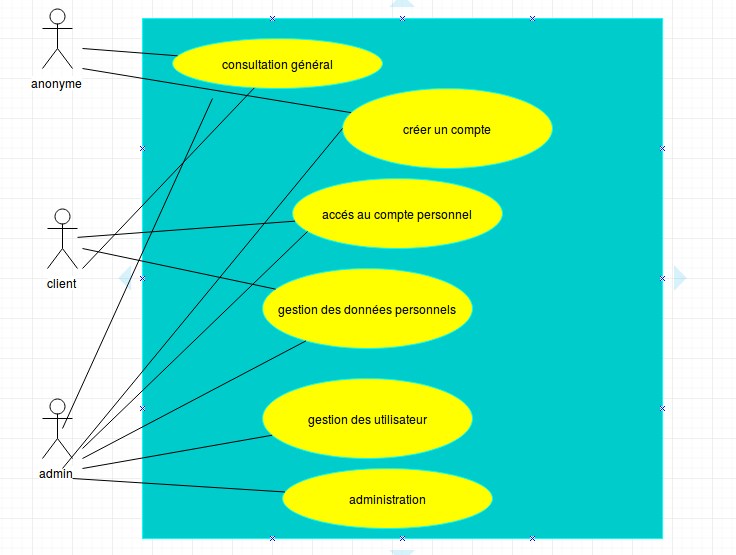
\includegraphics[width=300,height=250]{c3.png}}

\end{center}


\begin{center}
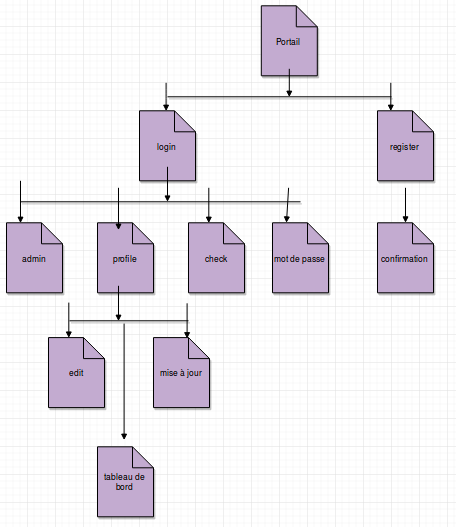
\includegraphics[width=300,height=250]{p3.png}}

\end{center}


\subsection{Modélisation}


\begin{center}
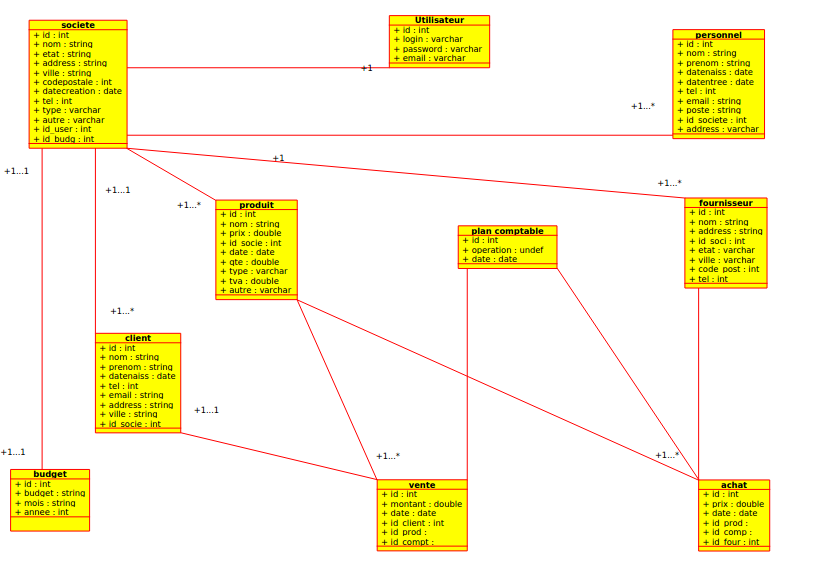
\includegraphics[width=300,height=250]{mod5.png}}

\end{center}



\subsection{Front-end}



\begin{center}
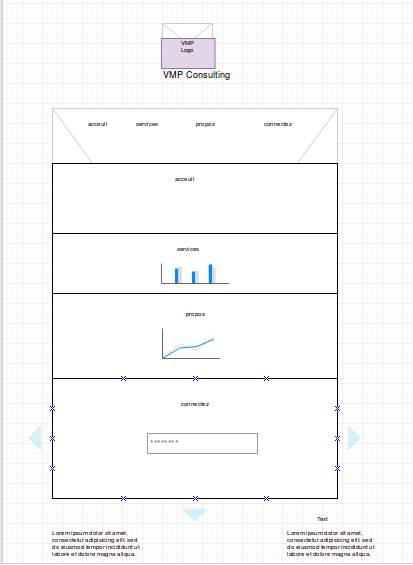
\includegraphics[width=300,height=250]{mod2.png}}

\end{center}

\subsection{Back-end}



\newpage

\section{Développement et Implémentation}

\subsection{Sécurité}

\subsection{Administration}

\subsection{Tableau de bord}

\subsection{Temps réel}

\subsection{Services}



\newpage

\section{Résultats}

\subsection{Démonstrations}

\begin{center}

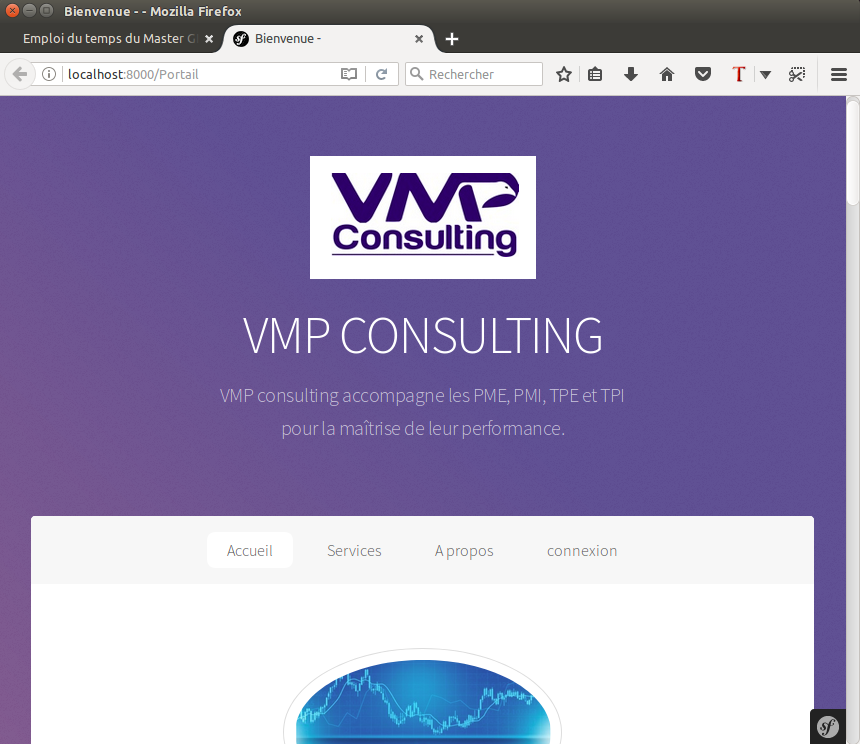
\includegraphics[width=300,height=250]{v1.png}} \\ \\
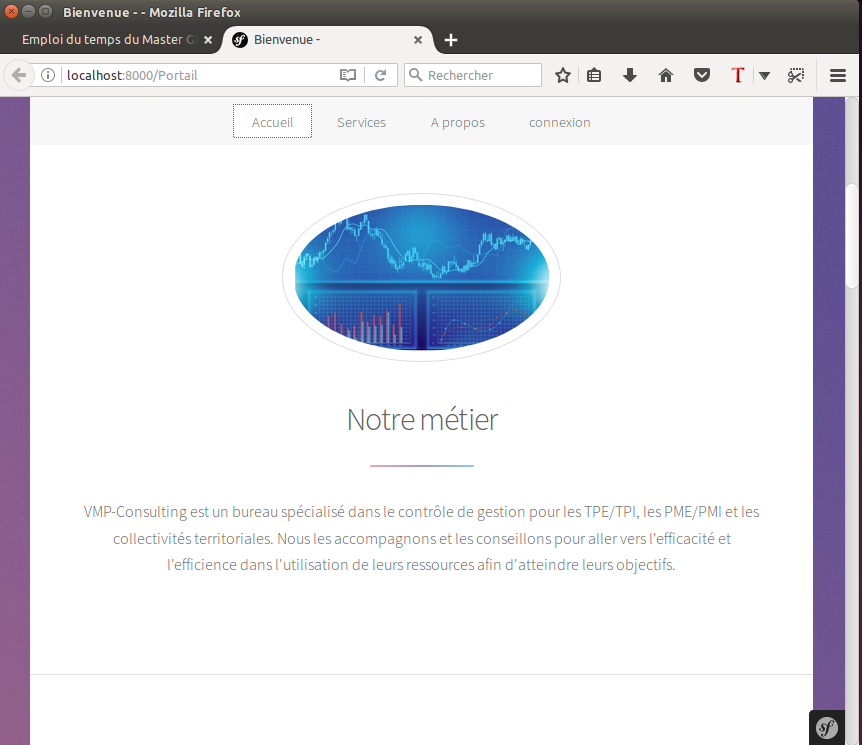
\includegraphics[width=300,height=250]{v2.png}} \\ \\
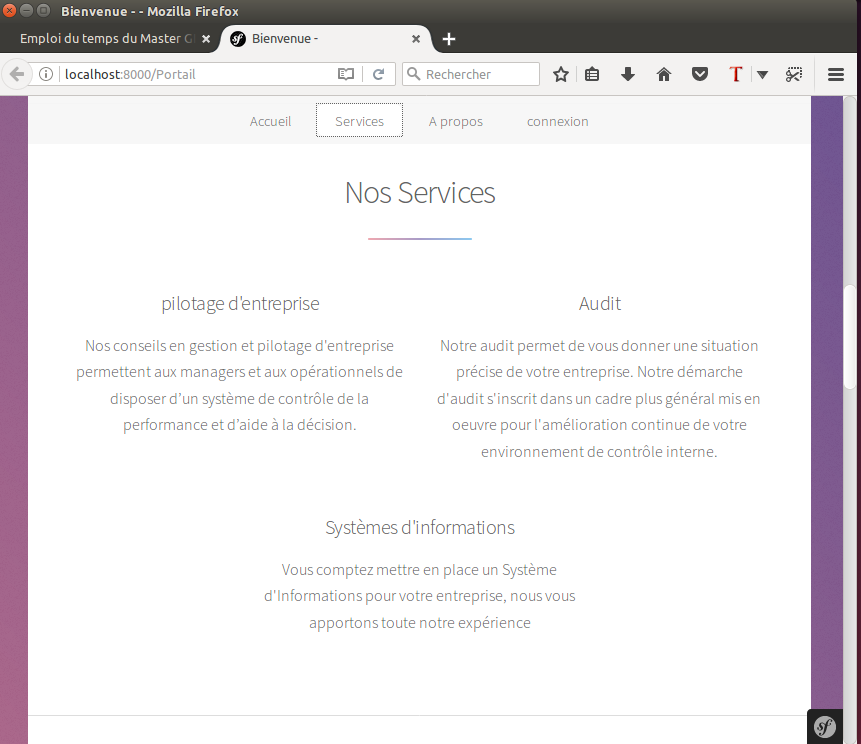
\includegraphics[width=300,height=250]{v3.png}} \\ \\
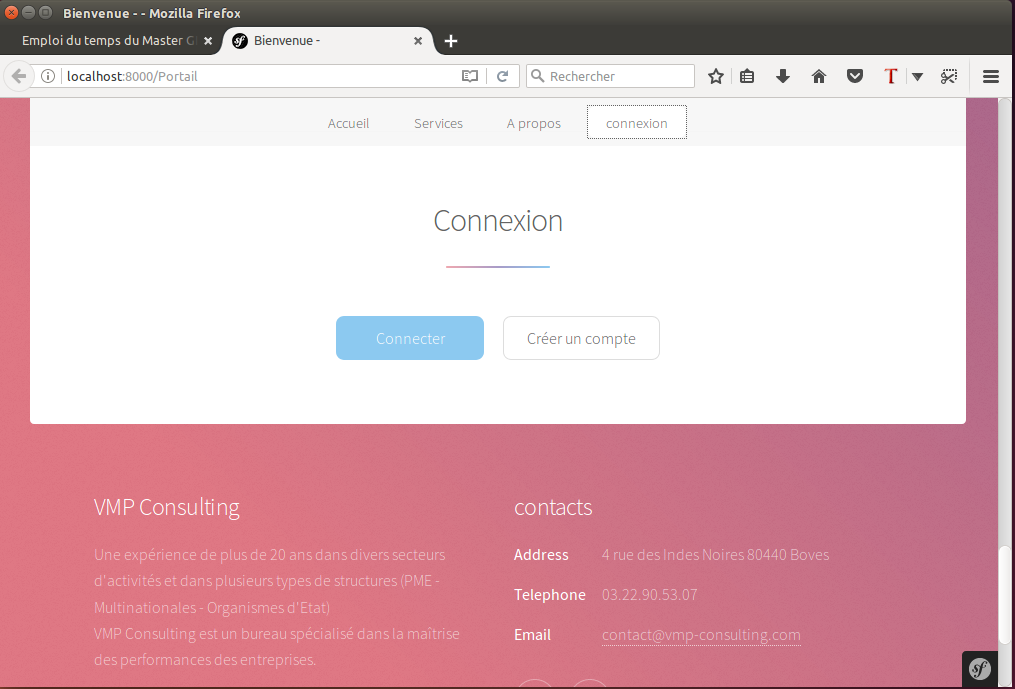
\includegraphics[width=300,height=250]{v4.png}} \\ \\
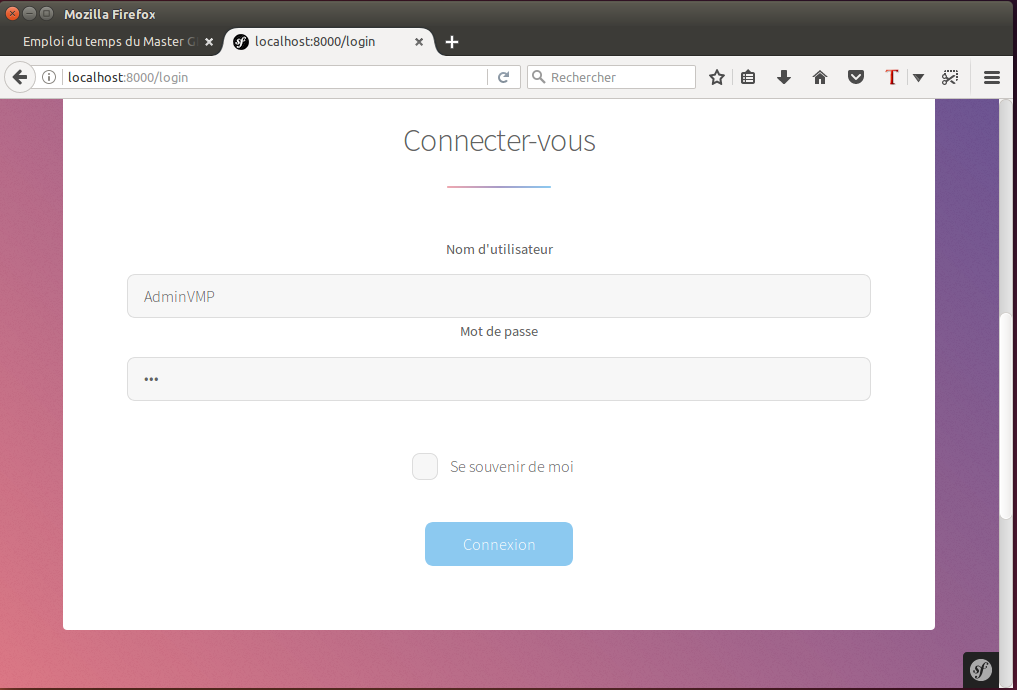
\includegraphics[width=300,height=250]{v5.png}} \\ \\
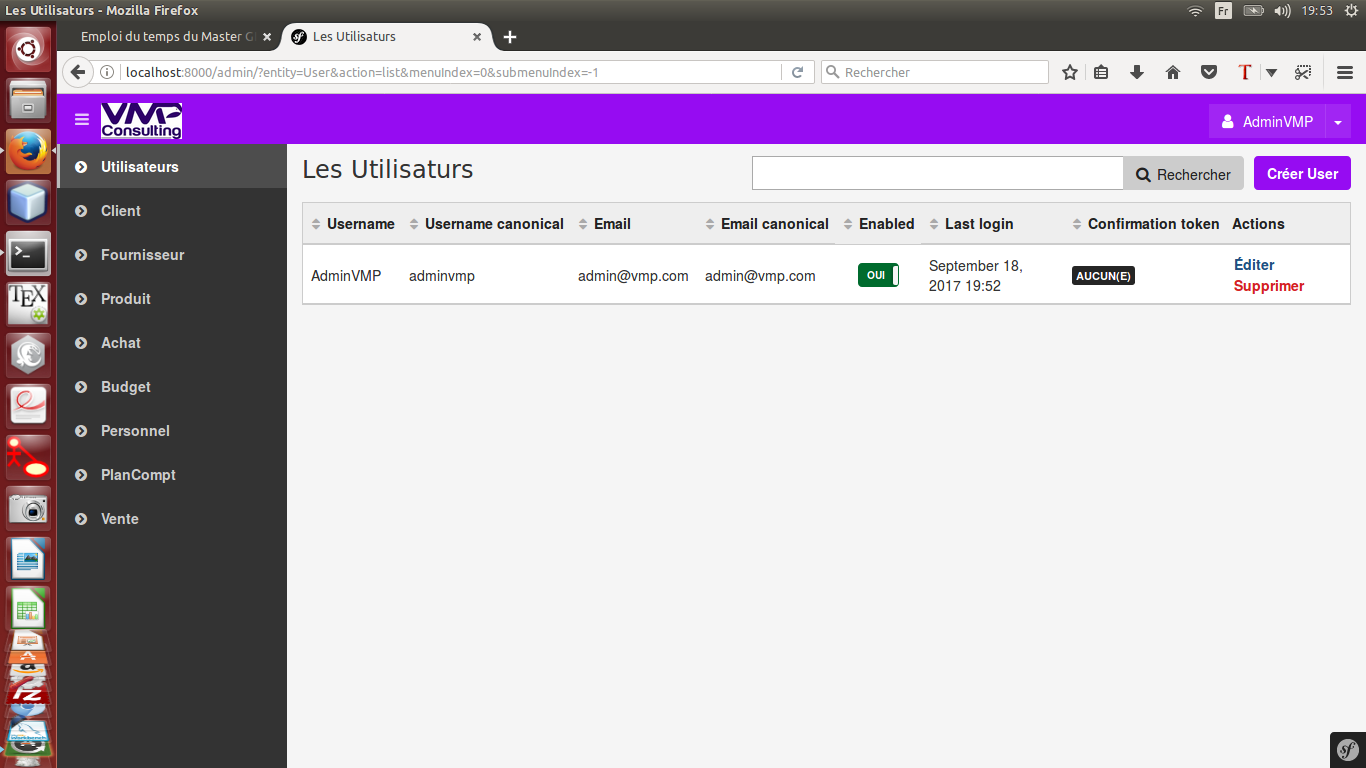
\includegraphics[width=300,height=250]{v6.png}} \\ \\
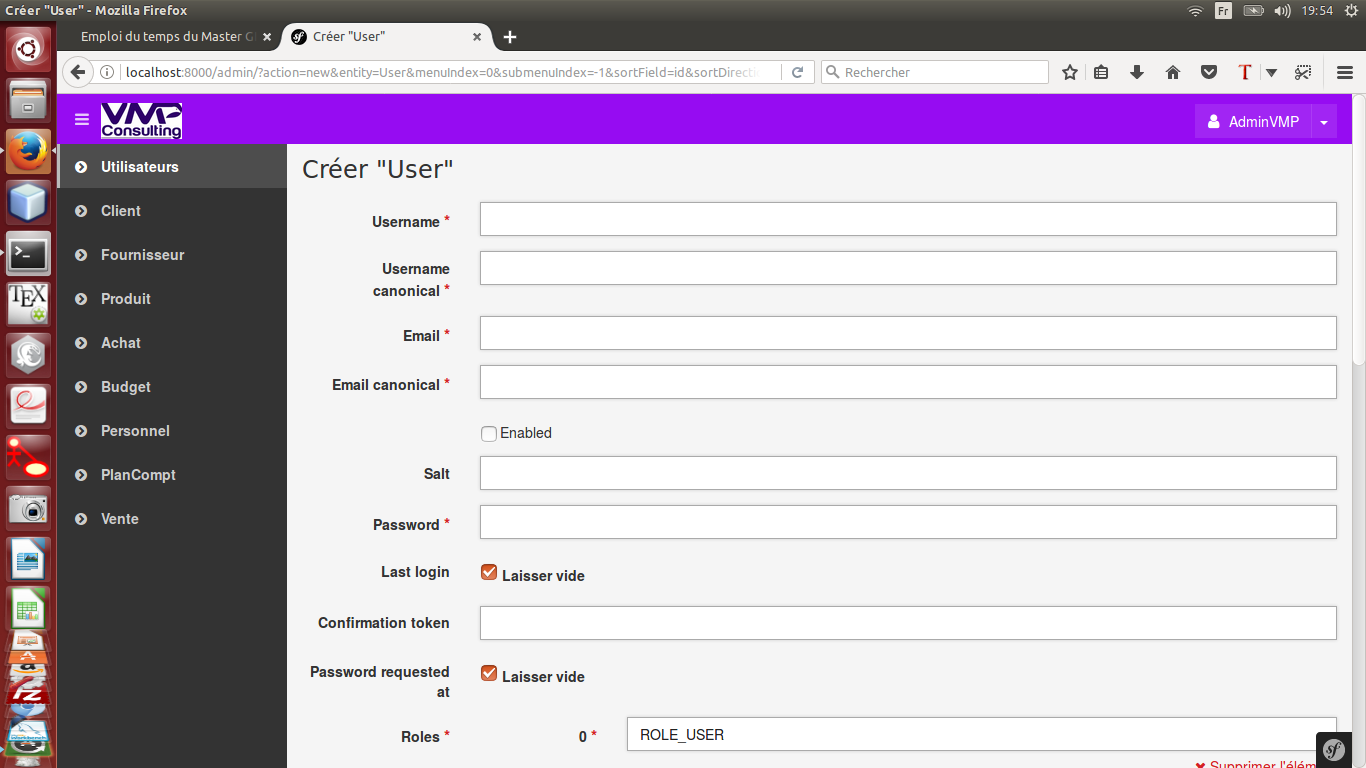
\includegraphics[width=300,height=250]{v7.png}} \\ \\
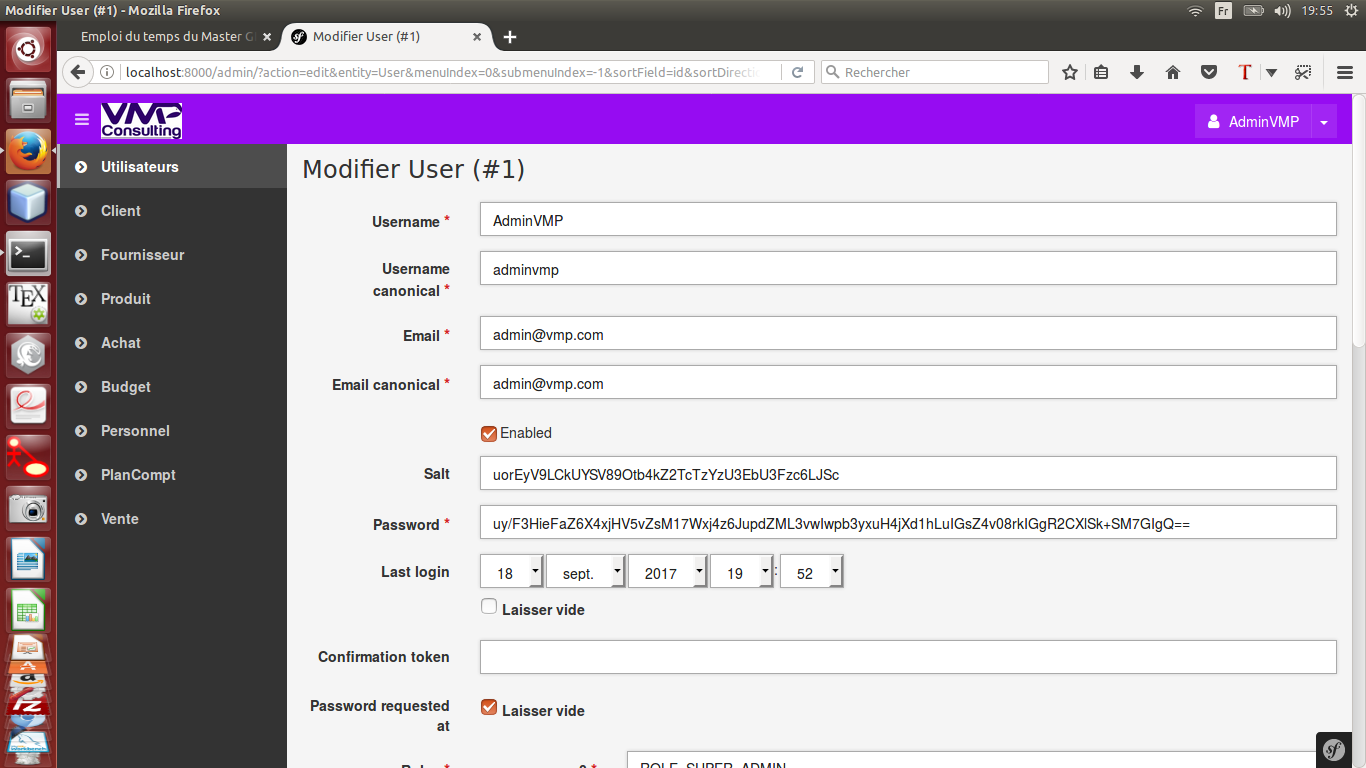
\includegraphics[width=300,height=250]{v8.png}} \\ \\
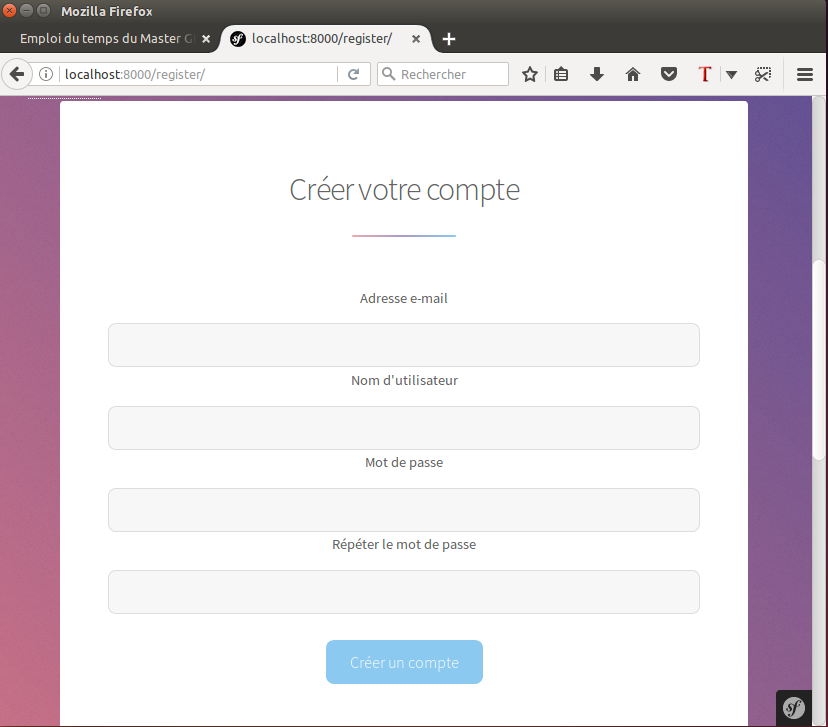
\includegraphics[width=300,height=250]{v9.png}} \\ \\
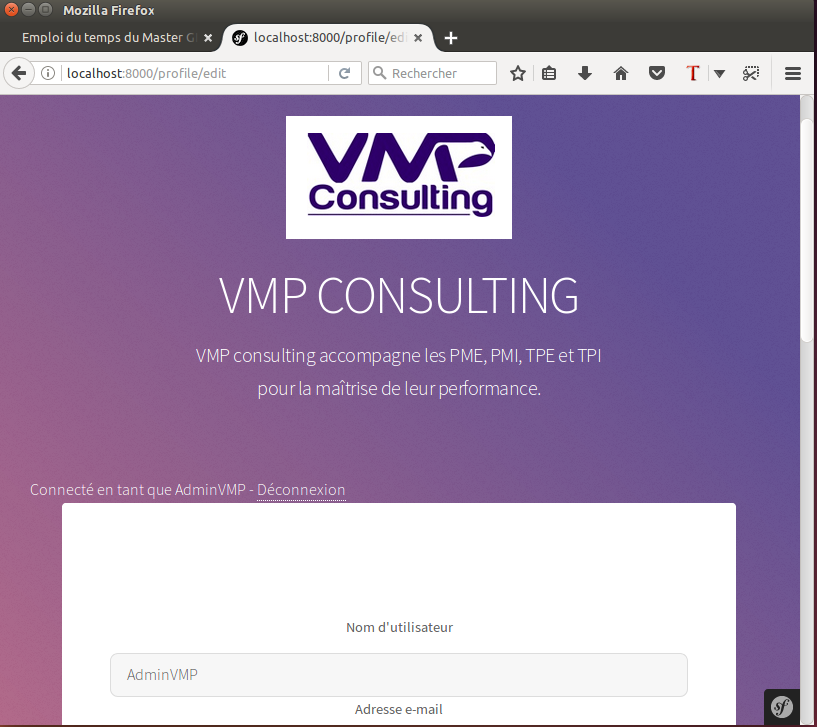
\includegraphics[width=300,height=250]{v10.png}} \\ \\

\end{center}

\subsection{Bilan}



\newpage
\section{Conclusion}


\newpage
\section{Bibliographie}

\newpage
\section{Annexe}
		
\end{document}
